\chapter{架构、时间尺度与数据合同}
\label{ch:arch}

本章要判定的量是：信息是否只沿规定的接口流动。判定失败的表现是品质估计直接断电，或安全测量被送进网络特征，或模块之间传递一个不带不确定度的均值。

这些接口装在同一台蒸烤一体机上。加热、蒸汽、排汽和风机是唯一的执行器出口。表面温度、腔温和质量从食品侧进入。水位、管温、门、腔压和剩余电流从安全侧进入。两侧不共用一根信号线，所以品质模型的错误不能改写断电条件。

\section{闭环}

\paragraph{要判定的量}
边界、观测、后验、信息动作、品质动作、结构方程和安全投影是否接成一个环，并且真值场不从侧面进入在线模块。

\paragraph{继承的文献层与不继承的层}
继承估计与预测控制的分离 \cite{rawlings2017}，以及屏障在参考动作之后 \cite{ames2017cbf}。不继承把学习模块放进安全环。不继承两套互不相同的参数：因果层与优化层读取同一后验。

\begin{figure}[ht]
\centering
\begin{tikzpicture}[
  node distance=6mm and 8mm,
  box/.style={draw, rounded corners, align=center, font=\small, inner sep=3pt, minimum width=28mm},
  arr/.style={-{Stealth}, thick}
]
\node[box] (w) {食品与腔体\\边界};
\node[box, right=of w] (y) {可安装观测};
\node[box, right=of y] (e) {联合后验};
\node[box, below=of e] (a) {对偶动作\\信息或品质};
\node[box, right=of e] (c) {结构方程\\路径效应};
\node[box, below=of c] (u) {测量隔离\\安全投影};
\node[box, left=of u] (m) {有限时域\\品质优化};
\draw[arr] (w)--(y);
\draw[arr] (y)--(e);
\draw[arr] (e)--(c);
\draw[arr] (c)--(m);
\draw[arr] (m)--(u);
\draw[arr] (u.west) -- ++(-2.2,0) |- (w.south);
\draw[arr] (e)--(a);
\draw[arr] (a.west) -- ++(-1.6,0) |- (w.east);
\end{tikzpicture}
\caption{闭环的依存关系图，不是测量。信息动作与品质动作在投影之前分开计算，进入同一个执行器接口。}
\end{figure}

已运行核把这个环收成一个时间步里的顺序：读表面温度和平均含水，更新热阻代理和冷点估计，形成加热请求，用加热器温度削减请求，再推进十六条控制体。结构方程和有限时域优化不在这个顺序里。图中的那些框是规格；核是规格的一条退化路径。

\begin{figure}[ht]
\centering
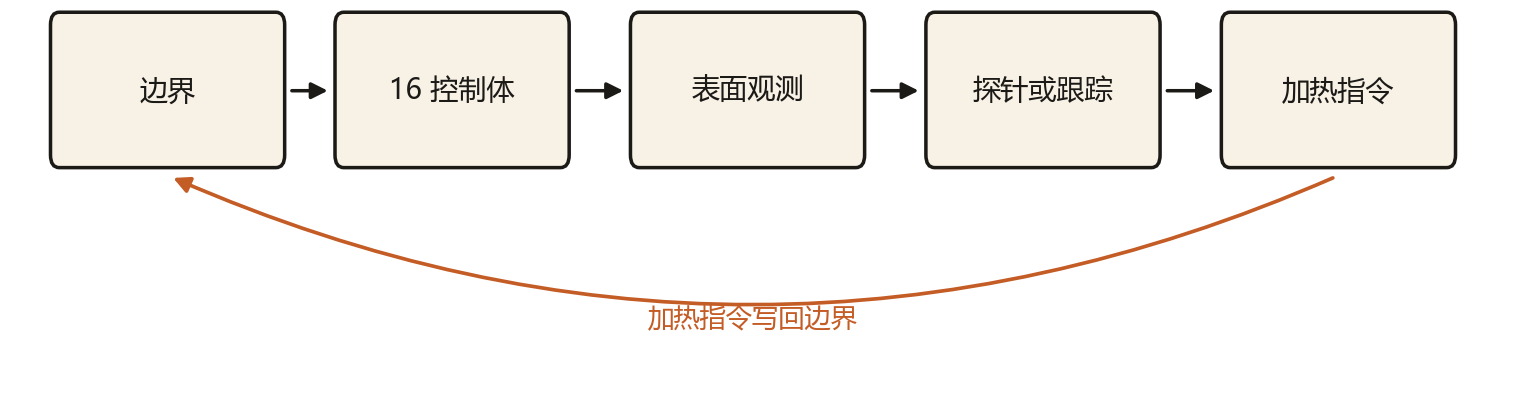
\includegraphics[width=\textwidth]{paper/M_loop.png}
\caption{评分核里实际走通的五段。加热指令回到边界。结构方程、集合滤波和预测控制求解器不在这五段里。}
\end{figure}

\begin{figure}[ht]
\centering
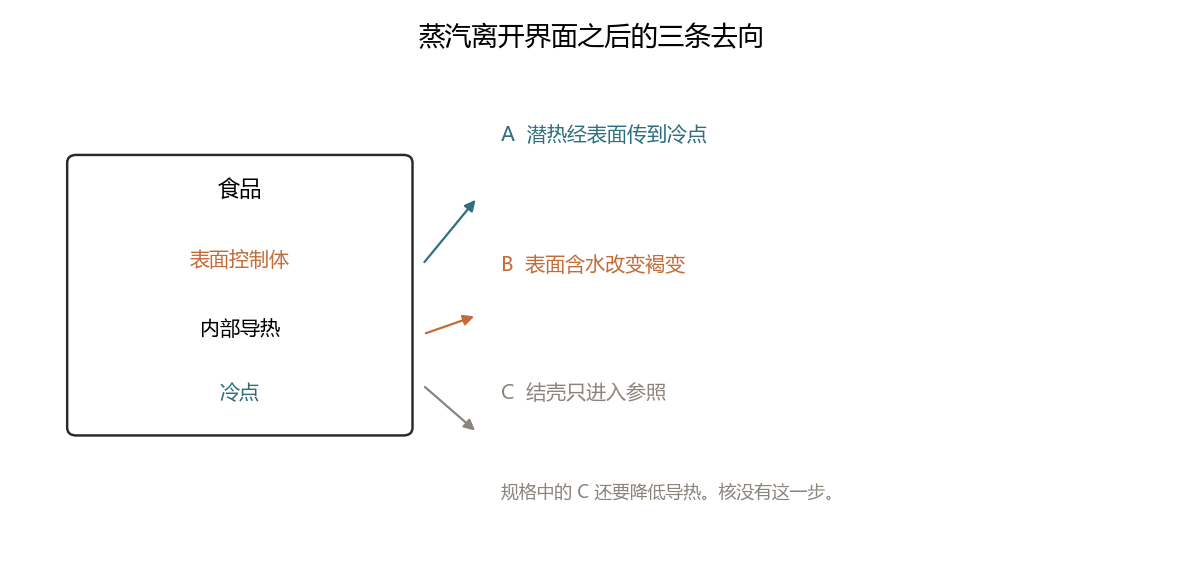
\includegraphics[width=0.92\textwidth]{paper/M_paths.png}
\caption{蒸汽离开表面之后，规格里有三条去向。核里路径 C 只进入热阻参照，不改变控制体导热。}
\end{figure}

\paragraph{本节不能推出的结论}
画出闭环不能推出每一步都有独立进程。合同约束的是数据依赖，不是部署拓扑。

\section{五层}

\paragraph{要判定的量}
每一层的输入里是否含有它不该读的对象。含有则该层的输出不能进入下一层。

\begin{description}
\item[L1 过程] 腔体几何、加热、蒸汽、风机、食品几何与初始场。仿真中由积分器充当。该层不含估计。本次积分器没有单独的腔体流动场。
\item[L2 多尺度模型] 把过程压缩为决策状态的演化。压缩必须保留冷点、表面干耗和局部过热。十六条控制体保留了冷点（最低温度）和表面温度，没有保留温度标准差的决策项。
\item[L3 结构孪生] 保存父节点固定的结构方程和参数后验。本次核没有这一层的积分。
\item[L4 对偶决策] 计算信息价值、品质价值，并选择动作。学习模块只允许在这一层。本次对偶策略是固定时间窗加饱和线性请求，不是信息增益的最大化。
\item[L5 安全执行] 电气、热、腔压、门封，以及只依赖这些测量的投影。这一层不调用网络。本次只有加热器温度进入削减。
\end{description}

执行器接口只有一个。动作进入接口之前带有标记：信息、品质或降级保温。标记决定它来自哪一个目标函数，不决定它能否绕过投影。核里的模式整数 \(0,1,2\) 就是这个标记的退化形式：品质、探针、保持。保持时请求降到 \(0.15\)，仍然经过同一条加热器更新。

\paragraph{本节不能推出的结论}
五层划分不能推出 L4 的网络已经训练。学习模块缺席时，L4 必须退回声明过的物理降阶，而不是保留上一次网络输出。

\section{四个时间尺度}

\paragraph{要判定的量}
慢计算是否能够关闭快保护。若能，架构不成立。

\begin{table}[ht]
\centering
\caption{尺度及允许的计算}
\begin{tabularx}{\textwidth}{llX}
\toprule
尺度 & 量级 & 允许的计算 \\
\midrule
电气切断 & 毫秒至 10 ms & 漏电、过流，无处理器 \\
热安全 & 0.1--1 s & 超温、干烧、腔压 \\
估计与动作 & 1--5 s & 滤波、信息价值、一次动作 \\
品质演化 & 10 s 至数十分钟 & 反应进度与预测时域 \\
跨次更新 & 一次过程结束 & 精度提高才写回类别先验 \\
\bottomrule
\end{tabularx}
\end{table}

快环可以中断慢环。慢环不能关闭快环。学习模块超时，则保持上一次已经投影的执行量，不保持网络的最后一次原始输出。

界面冷凝、蒸发的时间尺度是秒，冷点导热的时间尺度是分钟。动作设计利用这个分离：短脉冲改变表面节点，几乎不推动冷点进度。附录 \ref{app:scales} 用 \(\alpha=2.0\times 10^{-7}\,\mathrm{m}^2/\mathrm{s}\) 和 40 s 窗口算出 30 mm 的 Fourier 数为 \(8.9\times 10^{-3}\)。种子 7 的冷点在这 40 s 内从 \(8.01^\circ\mathrm{C}\) 到 \(8.05^\circ\mathrm{C}\)，与这个分离同方向。同方向不是对真实食品扩散率的测定。

本次时间步是 2 s，落在“估计与动作”的量级里，没有毫秒级的漏电回路。因此电气切断是规格，不是这次步进已经包含的动力学。

\begin{figure}[ht]
\centering
\begin{tikzpicture}[
  box/.style={draw, rounded corners, align=center, font=\small, inner sep=3pt, minimum width=32mm},
  arr/.style={-{Stealth}}
]
\node[box] (e) {电气切断};
\node[box, right=8mm of e] (h) {热安全};
\node[box, right=8mm of h] (a) {估计与动作};
\node[box, right=8mm of a] (q) {品质演化};
\draw[arr] (e)--(h);
\draw[arr] (h)--(a);
\draw[arr] (a)--(q);
\draw[arr, dashed] (h.south) -- ++(0,-0.6) -| (e.south);
\end{tikzpicture}
\caption{时间尺度的依存关系图，不是测量。实线是允许的调用方向。虚线表示快环可以中断慢环；慢环没有指向快环的关闭边。}
\end{figure}

\paragraph{本节不能推出的结论}
尺度分离不能推出任意短的蒸汽都无害。表面褐变和表面浸湿仍要进损伤预算。预算约束的是 \(\alpha_b\) 和 \(\varepsilon_{l,s}\)，不是冷点温度是否“看起来没变”。

\section{模块合同}

\paragraph{要判定的量}
模块之间传递的是分布还是一个点。把均值当成确定值，合同视为被破坏。

\begin{center}
\begin{tabularx}{\textwidth}{llX}
\toprule
模块 & 读入 & 写出 \\
\midrule
\texttt{sensor\_bus} & 物理量时序 & 带时间戳和不确定度的观测 \\
\texttt{manifold} & 观测、类别先验 & 集合或混合后验 \\
\texttt{dual\_policy} & 后验、执行器约束 & 标记过的动作 \\
\texttt{causal\_twin} & 后验、候选干预 & 轨迹与路径差 \\
\texttt{shield} & 候选动作、安全测量 & 投影后的执行量 \\
\texttt{knowledge} & 充分统计量 & 仅当精度提高时的新先验 \\
\bottomrule
\end{tabularx}
\end{center}

本次核没有这些模块名。对应关系是：观测在时间步内现场生成；后验退化成一个 \(\hat r\)、一个方差和一个 \(\hat T_c\)；策略直接写请求；没有因果模块；加热器削减代替投影；没有跨次写回。退化之后，下游仍然不应该把 \(\hat T_c\) 当成真值冷点。种子 7 在 1200 s 时估计 \(63.8^\circ\mathrm{C}\)、冷点 \(46.7^\circ\mathrm{C}\)，估计高于冷点。停机判据若把估计当成真值，就会在进度未到设计线时转入保持。该轨迹在 1680 s 正是这样：估计 \(85.85^\circ\mathrm{C}\)，冷点 \(73.0^\circ\mathrm{C}\)，\(\alpha_m=0.755\)。

\paragraph{本节不能推出的结论}
合同表不是软件目录已经实现的证明。缺模块时，正文只能写规格和退化路径，不能写该模块的误差指标。

\section{腔体上的最小执行与观测}

\paragraph{要判定的量}
信息动作是否需要额外机械机构。若不需要，探针必须能由已有的加热、蒸汽、热风和排汽组成。

\paragraph{继承的文献层与不继承的层}
继承的是边界条件进入食品的方式：对流、辐射和相变潜热 \cite{datta2007}。不继承某一腔体的风道尺寸。不继承把穿刺探针列为系统可重构性的必要条件。

过程载体是同一腔体内可切换的背部或顶部加热、蒸汽入口、热风、排汽阀。被动观测为腔温、腔湿、排气温度、加热功率、蒸汽功率与水位、门状态、漏电、壳体温度。食品侧为底部质量、门侧热像或一维热电堆。穿刺温度只作为对照通道。

蒸与烤的执行器已经覆盖短时边界组合。P4 的两段——先冷凝方向、再排汽高风——不增加阀门，只改变已有阀门的目标函数和时序。湿度调节最小化湿度误差；信息动作最大化参数信息。日志要记录这一时刻哪一个函数产生了指令。

本次核的执行量是加热、蒸汽和风机三个数。排汽没有独立变量，它被吸收进“蒸汽关闭且风机升高”。水位、门、漏电、腔压没有状态。因此“最小执行”在核里只覆盖加热与气流两路的一部分。

\paragraph{本节不能推出的结论}
执行器种类足够，不能推出探针库已经在线打分。固定时间窗是库的一个元素的时间表，不是 \(\argmax(G-\lambda C)\)。
